\section{Proof of the main theorem}\label{sec:twoside}

\subsection{Notation and a preliminary lemma}

We will use the same set of definitions for bad events and increase sets that we did in \cref{sec:overview} for polygons without inside atoms. For the benefit of the reader we repeat them here. Recalling the definitions from \cref{sec:polynotation}, partition each set $\delta(S)$ into three sets $E^\leftarrow(S), E^\rightarrow(S)$ and $E^\circ(S)$ such that
 \begin{align*}
 	E^\leftarrow(S) &= E(S \cap S_L, S_L \smallsetminus S) \\
 	 E^\rightarrow(S) &= E(S \cap S_R, S_R \smallsetminus S) \\
 	 E^\circ(S) &= \delta(S) \smallsetminus (E^\leftarrow(S) \cup E^\rightarrow(S))
 \end{align*}
In addition we define the left and right bad events:
\begin{align}
	B^\rightarrow (p) &= \mathbb{1}\{|E^{\rightarrow} (L(p)) \cap T|\ne 1\text{ or }|E^\circ (L(p)) \cap T|\ne 0\}\notag\\
B^\leftarrow (p) &= \mathbb{1}\{|E^{\leftarrow} (R(p)) \cap T|\ne 1\text{ or }|E^\circ (R(p)) \cap T|\ne 0\}. \label{defn:badevents2}
\end{align}
If $L(p)$ does not exist, simply assume the left bad event never occurs, and similarly if $R(p)$ does not exist assume the right bad event never occurs.

Define $L(p)^{\cap R} := L(p) \cap L(p)_R$, and let $L^*(p) \in \cC$ be the cut crossing $L(p)^{\cap R}$ on the left that {\em maximizes}  $|O(L^*(p) \cap L(p)^{\cap R})|$ (and similarly $R^*(p)$ to maximize the intersection with $O(R(p)^{\cap L})$ on the right). If $L^*(p)$ does not exist, i.e. no cut crosses $L(p)^{\cap R}$ on the left, set $L^*(p) = \emptyset$, and similarly for $R^*(p)$. We let:

\begin{figure}[htb]\centering
	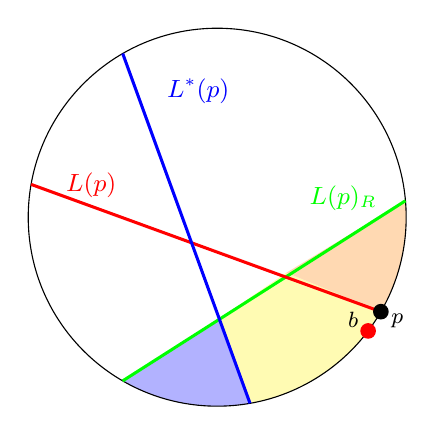
\begin{tikzpicture}[scale=0.8]
		\fill [color=blue!30] (240:3) -- (0.03,-1.61) -- (280:3)  arc (280:240:3); 
		\fill [color=yellow!30] (280:3) -- (0.03,-1.61) -- (1.1,-0.88) -- (330:3) arc (330:280:3);
		\fill [color=orange!30] (330:3) -- (1.1,-0.88) -- (5:3) arc (365:330:3);
		\draw (0,0) circle (3);
		\draw [color=green,line width=1.1pt] (240:3) -- (5:3);
		\node [color=green] at (2,0.3) () {\small $L(p)_R$};
		\draw [color=red, line width=1.1pt] (170:3) --   (330:3);
		\node [color=red] at (-2,0.5) () {\small $L(p)$};
		\draw [color=blue,line width=1.1pt] (120:3) -- (280:3);
		\node [color=blue] at (-0.3,2) {\small $L^*(p)$};
		\node [color=black,circle,fill=black,inner sep=2] at (330:3) () {};
		\node at (330:3.3) () {\footnotesize$p$};
		\node [circle,fill=red,inner sep=2] at (323:3) {};
		\node at (323:2.7) () {\footnotesize $b$};
	\end{tikzpicture}
	\caption{\small Recap of some basic definitions: $L(p)$ is the cut crossed on both sides with rightmost polygon point $p$ (and contains all atoms below the red diagonal. $L(p)_R$ is the cut crossing $L(p)$ on the right that minimizes the number of outside atoms in $L(p)^{\cap R} = L(p) \cap L(p)_R$, i.e., in yellow + blue.	Note that the cut $L(p)^{\cap R}$ contains all atoms in the yellow and blue regions (which may include inside atoms).  Since this region is the set difference of two $\eta$ near min cuts, it is a $2\eta$ near min cut. $L^*(p)$ is the cut crossing $L(p)^{\cap R}$ on the left that maximizes the number of outside atoms in the intersection, i.e., maximizes the number of outside atoms in the blue region. $E^\rightarrow (L(p))$ are the edges between atoms in the yellow region and atoms in the orange region. There is one edge in the tree that is in $E^\rightarrow (L(p))$ with probability $1-O(\eta)$ and when this event does not occur, $B^\rightarrow(p)$ occurs. ($B^\rightarrow(p)$ also occurs if $|E^\circ (L(p)) \cap T|\ne 0$.)}
\end{figure}

\begin{align}
	E(B^\rightarrow (p)) &:= E( L(p)^{\cap R} \smallsetminus L^*(p), L(p)_R \smallsetminus  L(p)^{\cap R})  \notag\\
	E(B^\leftarrow (p)) &:= E( R(p)^{\cap L} \smallsetminus R^*(p), R(p)_L \smallsetminus  R(p)^{\cap L})\label{defn:slackincrease2}.
\end{align}

The following important lemma is the generalization of \cref{claim:1} from \cref{sec:overview} to the case in which there may be inside atoms. It uses that by \cref{lem:extendedprop20} many regions of the polygon do not contain inside atoms.

%\Nathan{Check this next proof for clarity}

\begin{lemma}\label{lem:samerightEPsameedgeset}
	Let $A, B \in \cC_{2}$ such that $A=(a_1,a_r)$ and $B=(a_2,a_r)$ share a rightmost polygon point $p_r$. Then, $A_R = B_R$ and $E^\rightarrow(A) = E^\rightarrow(B)$.
\end{lemma}
\begin{proof}
	WLOG assume $A \subseteq B$. First, we will prove that if a cut $R$ crosses $A$ on the right, it also crosses $B$ on the right. So, let $R$ be a set crossing $A$ on the right. Then, since $R$ contains $a_{r}$, $R \cap B \not= \emptyset$. Furthermore, $R$ contains atom $a_{r+1}$, so $R \not\subseteq B$. Finally, $B$ contains $a_1$ since $A \subseteq B$ yet $R$ does not. Therefore, $R$ crosses $B$ on the right. 
	
	Therefore, by \cref{def:SLR} $A_R = B_R$ since the set of cuts crossing $B$ on the right is a superset of cuts crossing $A$ on the right and any cut which crosses $B$ but not $A$ contains all atoms of $A$, so would have a larger intersection with $O(B)$. (If two sets have the same intersection with $O(A)$ we use the same tie-breaking rule for both $A_R$ and $B_R$.)   
	
	Now we prove that $E^\rightarrow(A) = E^\rightarrow(B)$. Let $R=A_R=B_R$. It suffices to show that $R \cap A = R \cap B$ and $R \smallsetminus A = R \smallsetminus B$ because any edge $e \in E^\rightarrow(A)$ has one endpoint in $R \cap A$ and one in $R \smallsetminus A$. To obtain $R \cap A = R \cap B$ notice that $O(R \cap A) = O(R \cap B) \not= \emptyset$ and by \cref{lem:cutdecrement} $R \cap A, R \cap B$ are $2\eta$ near minimum cuts (since $R$ crosses both $A$ and $B$), so by \cref{lem:extendedprop20}, $R \cap A = R \cap B$. Similarly to obtain $R \smallsetminus A = R \smallsetminus B$ notice that $O(R \smallsetminus A) = O(R \smallsetminus B) \not= \emptyset$ and $R \smallsetminus A, R \smallsetminus B$ are $2\eta$ near min cuts so by  \cref{lem:extendedprop20} we have $R \smallsetminus A = R \smallsetminus B$. 
	\end{proof}

\subsection{Main theorem}

The following is the main technical result of the paper:
\begin{restatable}[Main theorem]{theorem}{maintheorem}\label{thm:cutsbothsideswithinside}
Let $x^0$ be a feasible LP solution of \eqref{eq:tsplp} with support $E_0=E\cup \{e_0\}$ and let $x$ be $x^0$ restricted to $E$.  For {\em any} distribution $\mu$ of spanning trees with marginals $x$,  $0<\eta \leq 1/10$ and $\alpha > 0$, there is a random vector $s^*:E \to \R_{\geq 0}$ (the randomness in $s^*$ depends exclusively on $T\sim\mu$) such that
\begin{itemize}
%\item $\ys_{\es}\geq 1/4$ for all OPT edges $\es$,
\item For any $\eta$-near minimum cut $S$ which is crossed on both sides, if $\delta(S)_T$ is odd then $s^*(\delta(S)) \geq \alpha(1-\eta)$;
\item For any $e \in E$, $\E{s^*_{e}} \leq 18\alpha\eta x_e.$
\end{itemize}
\end{restatable}
%\begin{proof}[Proof of \cref{thm:cutsbothsideswithinside}]
%For any polygon point $p$, whenever $\cI(p)$  occurs, define $s^*_{e}=\alpha \decrease x_e $ for each $e \in I^\leftarrow(p) \cup I^\rightarrow(p)$. 
%By \cref{lem:everyedgetwocutnoinside},
%an edge $e=(a,b)$ is in at most one set $I^\leftarrow(p)$ and at most one set $I^\rightarrow(q)$ for points $p,q$ of the polygon. Then, by \cref{lem:OPT-edge-increase-prob-xed-both-sides},
%$$\E{s_{e^*}} \leq (\P{\cI(p)} + \P{\cI(q)})\frac{2+\eta}{1-\eta}\decrease x_e \leq (9\eta) \cdot 2\cdot \frac{2+\eta}{1-\eta}\decrease x_e =\frac{18\eta(2+\eta)}{1-\eta}\decrease x_e.$$
% On the other hand, for any $\eta$-near min cut $S=(p_l,p_r)$ that is crossed on both sides if $\delta(S)_T$ is odd, then by \cref{lem:xed-both-sides-one-increases} at least one of $\cI(p_l),\cI(p_r)$ occurs, so
%$$ s(\delta(S)) + s^*(\delta(S)) \geq  - x(\delta(S))\beta + s^*(I^\leftarrow(p_l))+s^*(I^\rightarrow(p_r)) \geq -(2+\eta)\decrease + \frac{2+\eta}{1-\eta}\decrease(1-\eta) = 0,$$
%where in the inequality we use \cref{lem:massinI}.
%\end{proof}
%
%\cref{lem:s-handle-cross} and \cref{lem:small-exp-cost-both-sides} together prove \cref{thmcutsbothsides}.

Our slack vector for the above theorem will be exactly as in \cref{sec:overview}. In particular, for  every bad event $B$ which occurs among those defined in \cref{defn:badevents2}, we will set $s^*(e) = \alpha x_e$ for all $e \in E(B)$, where $E(B)$ is defined as in \cref{defn:slackincrease2}. In order to extend the argument from \cref{sec:overview} to prove this theorem in the case in which the polygon contains inside atoms, we prove the following two lemmas from which the theorem follows easily:

\begin{restatable}[All cuts are satisfied]{lemma}{allcutssatisfied}\label{lem:xed-both-sides-one-increases} Let $S=(p_l,p_r)$ be a cut which is crossed on both sides. Then, if $\delta(S)_T \not=2$, at least one of $B^\leftarrow(p_l),B^\rightarrow(p_r)$ occurs.
\end{restatable}

\begin{restatable}[Every edge is mapped to a constant number of bad events]{lemma}{constantnumberevents}\label{lem:constant-num-events}
Let $p,q$ be two polygon points such that $e=\{a,b\}$ and $a \in L(p) \cap L(q)$. 
Then, $e \not\in E(B^\rightarrow(p)) \cap E(B^\rightarrow(q))$.
\end{restatable}

Before proving these statements, we will show how they imply our main theorem. First we gives proofs for \cref{claim:2} and \cref{claim:xvaluenoinside} (as the formal proofs were omitted in the overview):

\begin{lemma}\label{lem:OPT-edge-increase-prob-xed-both-sides}
For any polygon point $p$, $\P{B^\rightarrow(p)}\leq 4.5\eta$ and $\P{B^\leftarrow(p)}\leq 4.5\eta$.
\end{lemma}
\begin{proof}
We will prove this for $B^\rightarrow(p)$, $B^\leftarrow(p)$ follows similarly. To simplify notation we abbreviate $L(p)$ to $L$.
Since $L$ is crossed on both sides, $L_L, L_R$ are well defined. Since by \cref{lem:cutdecrement} $L_R\cap L, L_R\smallsetminus L$ are $2\eta$-near min cuts and $L_R$ is an $\eta$-near mincut with respect to $x$, by \cref{lem:treeoneedge}, $\P{E^\rightarrow(L)_T=1}\geq 1-2.5\eta$. %Similarly, $\P{E^\leftarrow(R)_T=1}\geq 1-2.5\eta$. %Similarly, $\P{E^\leftarrow(L)_T = 1}\geq 1-2.5\eta$.

On the other hand, since $L, L_L, L_R$ are $\eta$-near min cuts, by \cref{lem:nmcuts_largeedges}, $x(E^\rightarrow(L)), x(E^\leftarrow(L)) \ge 1-\eta/2$. Therefore 
$$x(E^\circ(L)) \le 2+\eta - x(E^\leftarrow(L)) - x(E^\rightarrow(L)) \le 2\eta.$$ 
It follows that $\P{E^\circ(L)_T = 0}\geq  1-2\eta$. %Similarly, $\P{E^\circ(R)_T = 0}\geq  1-2\eta$.
	Finally,	by the union bound, all events occur simultaneously with probability at least $1-4.5\eta$, which gives the lemma.
	\end{proof}
	
\begin{lemma}\label{lem:massinI}
	For any polygon point $p$, $x(E(B^\leftarrow(p))),x(E(B^\rightarrow(p)))\geq 1-\eta$
\end{lemma}
\begin{proof}
First, observe that $L^*(p)$ crosses $L(p)_R$.
Notice (where we use $\uplus$ to denote disjoint union):
$$ L(p)^{\cap R}\smallsetminus  L^*(p) \biguplus L(p)_R\smallsetminus L(p) = L(p)_R \smallsetminus L^*(p).$$
Therefore, by \autoref{lem:cutdecrement} $L(p)^{\cap R}\smallsetminus  L^*(p) \biguplus L(p)_R\smallsetminus L(p)$ is a $2\eta$ near mincut. 
So, by \autoref{lem:sub-NMC-shared}, $x(E(B^\leftarrow(p))\geq 1-\eta$. 

The proof for $x(E(B^\rightarrow(p)))$ is similar. 
 \end{proof}

\begin{proof}[Proof of \cref{thm:cutsbothsideswithinside}]
Our slack vector is defined as follows. Initialize $s^*(e) = 0$ for all edges $e$. Then for each polygon $P$, for each polygon point $p \in P$, whenever $B^\leftarrow(p)$  occurs, let $s^*_{e}=\alpha x_e $ for each $e \in E(B^\leftarrow(p)) $. Whenever $B^\rightarrow(p)$ occurs, let $s^*_{e}=\alpha x_e $ for each $e \in E(B^\rightarrow(p))$. 
	
Now we show the first condition of the theorem. Let $S=[p,q] \in \cC_2$ and suppose that $\delta(S)_T$ is odd. It appears in some polygon $P$. Then by \cref{lem:xed-both-sides-one-increases}, either $B^\leftarrow(p)$ or $B^\rightarrow(q)$ has occurred. Assume the former, the other case is similar. In this event, we set $s^*(e) = \alpha x_e$ for all $e \in E(B^\leftarrow(p))$. However, using \cref{lem:samerightEPsameedgeset}, we have
$$E(B^\leftarrow(p)) \subseteq E^\leftarrow(p) = E^\leftarrow(S)$$
Therefore, by \cref{lem:massinI} $s^*(S) \ge \alpha (1-\eta)$ as desired. 
	
Now we verify the second condition of the theorem. First note that by \cref{fact:edges-internal-to-one-poly}, for any edge $e$, there is at most one polygon $P$ such that $e$ does not have the root as one of its endpoints. Therefore, there is at most one polygon $P$ for which $s^*_e$ may be increased since if $e$ is adjacent to the root, $e \not\in E^\rightarrow(S),E^\leftarrow(S)$ for any set $S$ in its connected component. 

Now let $e=\{a,b\}$ for some polygon $P$ such that $a,b \not= r$. We show that there are at most two polygon points $p$ for which $e \in E(B^\rightarrow(p))$. Suppose otherwise and there are at least three such polygon points $p$. Since $E(B^\rightarrow(p)) \subseteq \delta(L(p))$ for each such point $p$, we have $e \in \delta(L(p))$, which implies that there are two polygon points $p,q$ such that one of $a$ or $b$, WLOG $a$, is in both $L(p)$ and $L(q)$ and $e \in E(B^\rightarrow(p)) \cap E(B^\rightarrow(q))$. However this contradicts \cref{lem:constant-num-events} since $e$ is in at most one such set. One can similarly show that there are at most two polygon points $p$ such that $e \in E(B^\leftarrow(p))$. Therefore, any edge $e$ is in $E(B)$ for at most four bad events $B$. 

By \cref{lem:OPT-edge-increase-prob-xed-both-sides}, each bad event occurs with probability at most $4.5\eta$. Therefore, by the union bound:
$$\E{s^*(e)} \le 4 \cdot 4.5\eta \alpha x_e = 18 \alpha \eta x_e,$$
which gives the second condition and completes the proof. 
\end{proof}



\subsection{All cuts are satisfied}

In this section we first prove the following from which \cref{lem:xed-both-sides-one-increases} will easily follow:

\begin{restatable}{lemma}{circsubset}\label{lem:circsubset} For $S=(p_l,p_r) \in \cC_2$,
$E^\circ(S) \subseteq E^\circ(L(p_r)) \cup E^\circ(R(p_l))$.	
\end{restatable}

Note that if $S=(p_l,p_r) \in \cC_2$ then $L(p_r)$ and $R(p_l)$ exist, because $S$ is a candidate for both.

Before giving the proof of this we show how it implies \cref{lem:xed-both-sides-one-increases}. 

\allcutssatisfied*
\begin{proof}
We prove by contradiction. Suppose none of $B^\leftarrow(p_l),B^\rightarrow(p_r)$ occur; we will show that this implies $\delta(S)_T = 2$. 

Let $R=R(p_l)$. By \cref{lem:samerightEPsameedgeset} we have $S_L = R_L$ and $E^\leftarrow(R) = E^\leftarrow(S).$
Similarly for $L=L(p_r)$ we have $E^\rightarrow(L)=E^\rightarrow(S)$.

Now, since $B^\leftarrow(p_l)$ has not occurred,
$$1 = E^\leftarrow(R)_T = E^\leftarrow(S)_T \text{ and } E^\circ(R)_T = 0$$
and since $B^\rightarrow(p_r)$ has not occurred,
$$1 = E^\rightarrow(L)_T =  E^\rightarrow(S)_T \text{ and } E^\circ(L)_T = 0$$
So, to get $\delta(S)_T=2$, it remains to show that  $T\cap E^\circ(S) = \emptyset$. By \cref{lem:circsubset}, we have $E^\circ(S) \subseteq E^\circ(L) \cup E^\circ(R)$, which gives the claim.
\end{proof}

To prove \cref{lem:circsubset} we first need the following:

%\begin{lemma}\label{lem:nointersectionLR}
%For $S=(a_l,a_r) \in \cC_2$, let $L \in \cC$ cross $S$ on the left and $R \in \cC$ cross $S$ on the right. Then, $(L \smallsetminus S) \cap (R \smallsetminus S) = \emptyset$. 	
%\end{lemma}
%\begin{proof}
%	Suppose $(L \smallsetminus S) \cap (R \smallsetminus S) \not= \emptyset$. We will show that $L,R,S$ form a 3-cycle (\cref{def:kcycle}) which cannot exist. To show this (using that the root atom $r \not\in S \cup L \cup R$), it is enough to prove that all pairs cross and none of the three sets is a superset of the intersection of the two others. First, by assumption $L$ and $R$ cross $S$. $L$ and $R$ cross because $a_r \in R \smallsetminus L, a_l \in L \smallsetminus R$, so neither is a subset of the other, and because we assumed $(L \smallsetminus S) \cap (R \smallsetminus S) \not= \emptyset$ their intersection is nonempty. 
%	
%	In addition, we have $S \cap L \not\subseteq R$ because $a_l \in S \cap L$ but not in $R$. Similarly $S \cap R \not\subseteq L$. Finally, $L \cap R \not\subseteq S$ by the assumption $(L \smallsetminus S) \cap (R \smallsetminus S) \not= \emptyset$. Therefore $S,L,R$ form a 3-cycle which is a contradiction.
%\end{proof}
%
%\begin{corollary}\label{cor:nointersectionLR}
%	Let $A=(a_l,a_r),B=(a_{l'},a_{r'}) \in \cC_2$ such that $B$ crosses $A$ on the right and suppose $L$ crosses $A$ on the left and $R$ crosses $B$ on the right. Then, $(L \smallsetminus (A \cup B)) \cap (R \smallsetminus (A \cup B)) = \emptyset$. 
%\end{corollary}
%\begin{proof}
%To obtain this, first notice that since $A$ and $B$ cross, $A \cup B$ is a $2\eta$ near min cut. First we show $L$ crosses $A \cup B$, and by \cref{lem:OABcross} this will imply that $O(L)$ crosses $O(A \cup B)$. 
%
%To see this, since $L$ crosses $A$ on the left, $L$ contains the outside atom immediately to the left of $a_l$. However, $B$ cannot contain this atom since it crosses $A$ on the right. The remaining properties verifying that $L$ crosses $A \cup B$ follow from the fact that $L$ crosses $A$.
%
%Similarly we will have that $R$ crosses $A \cup B$. Given this, we can follow the same proof as the above and show that $A \cup B, L, R$ form a 3-cycle which cannot exist by \cref{lem:no-kcycle} since $\eta \le 1/3$. 
%\end{proof}

\begin{corollary}\label{cor:leftrightemptyextended}
	For all sets $S \in \cC_2$, we have $E^\leftarrow(S) \cap E^\rightarrow(S) = \emptyset$. Similarly, for all sets $A,B \in \cC_2$ such that $B$ crosses $A$ on the right, $E^\leftarrow(A) \cap E^\rightarrow(B) = \emptyset$. 
\end{corollary}
\begin{proof}
To see the first claim, suppose $S_L$ crosses $S$ on the left and $S_R$ crosses $S$ on the right, by \cref{lem:nointersectionLR} $(S_L \smallsetminus S) \cap (S_R \smallsetminus S) = \emptyset$. Since every edge in $E^\leftarrow(S)$ has an endpoint in $S_L \smallsetminus S$ and every edge in $E^\rightarrow(S)$ has an endpoint in $S_R \smallsetminus S$, this proves the claim. 	

A similar argument using \cref{lem:nointersectionLR} proves the second claim.
\end{proof}

Now we can prove the main lemma: 

\begin{figure}[htb]\centering
	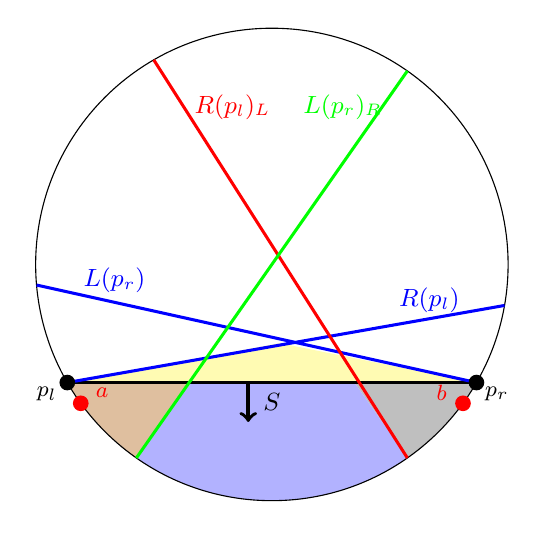
\begin{tikzpicture}
		\fill [color=brown!50] (210:3) -- (-1.05,-1.5) -- (235:3) arc (235:210:3);
		\fill [color=gray!50] (305:3) -- (1.05,-1.5) -- (330:3) arc (330:305:3);
		\fill [color=yellow!30] (210:3) -- (0.1,-1) -- (330:3);
		\fill [color=blue!30] (235:3) -- (-1.05,-1.5) -- (1.05,-1.5) -- (305:3) arc (305:235:3);
		\draw (0,0) circle (3);
		\draw [color=black,line width=1.1pt] (210:3) -- node [below] {\small$S$} (330:3);
		\draw [color=black,line width=1.3pt,->] (-0.3,-1.5) -- +(0,-0.5);
		\draw [color=blue,line width=1.1pt] (185:3) -- (330:3)
		(210:3) -- (350:3);
		\draw [color=red,line width=1.1pt] (120:3) -- (305:3);
		\draw [color=green,line width=1.1pt] (55:3) -- (235:3);
		\node [color=blue] at (-2,-0.2) () {\small$L(p_r)$};
		\node [color=blue] at (2,-0.45) () {\small$R(p_l)$};
		\node [color=red] at (-0.5,2) () {\small$R(p_l)_L$};
		\node [color=green] at (0.9,2) () {\small$L(p_r)_R$};
		\node [color=red,fill=red,circle,inner sep=2] at (216:3) () {};
		\node [color=red,fill=red,circle,inner sep=2] at (324:3) () {};
		\node at (210:3.3) () {\footnotesize $p_l$};
		\node [color=black,circle,fill,inner sep=2] at (210:3) () {};
		\node at (330:3.3) () {\footnotesize $p_r$};
		\node [color=black,circle,fill,inner sep=2] at (330:3) () {};
		\node [color=red] at (217:2.7) () {\footnotesize $a$};
		\node [color=red] at (323:2.7) () {\footnotesize $b$};
	\end{tikzpicture}
	\caption{Here we have a set $S$ which is crossed on both sides. We use in \cref{lem:circsubset} that $L(p_r) \cap R(p_l) = S$; in other words, the yellow region is empty.}
\end{figure}


\circsubset*
\begin{proof}
	For convenience, let $L=L(p_r)$ and $R=R(p_l)$. First suppose we had $L = S$ or $R = S$. In this case, by definition $E^\circ(S) = E^\circ(L)$ or $E^\circ(R)$, and we are done. So assume that $S \subsetneq L, R$. Therefore, $L$ and $R$ cross.  
	
	Now, notice that since $O(L \cap R) = O(S)$, by \cref{lem:extendedprop20}, we have $L \cap R = S$. This implies
	$\delta(S) \subseteq \delta(L) \cup \delta(R)$. To see this, let $e$ be an edge in $\delta(S)$. Then, it has an endpoint in both $L$ and $R$. However, its other endpoint is in $\overline{S} = \overline{L \cap R}$, and therefore cannot be in both $L$ and $R$ which implies it is in $\delta(L)$ or $\delta(R)$.  

	Now, by way of contradiction, suppose there exists an edge $e \in E^\circ(S)$ such that $e \not\in E^\circ(L) \cup E^\circ(R)$. Since $E^\leftarrow(S) = E^\leftarrow(R)$, $E^\rightarrow(S) = E^\rightarrow(L)$, and $e \in \delta(L) \cup \delta(R)$, it must be that $e \in E^\leftarrow(L) \cup E^\rightarrow(R)$. Since $L$ and $R$ cross, by \cref{cor:leftrightemptyextended} $e$ is in exactly one of $E^\leftarrow(L),E^\rightarrow(R)$; assume that $e \in E^\leftarrow(L)$ but not in $E^\rightarrow(R)$, the other case is similar. Therefore $e \not\in \delta(R)$, since it is not in $E^\leftarrow(R), E^\circ(R)$ or $E^\rightarrow(R)$. 
	
	However, $L_L$ crosses $L$ on the left and $R$ crosses $L$ on the right. Therefore, by \cref{lem:nointersectionLR}, we have $(L_L \smallsetminus L) \cap (R \smallsetminus L) = \emptyset$. However $e$ has one endpoint in $L \cap R = S$, one in $R \smallsetminus L$ (since $e \not\in \delta(R), e \in \delta(L)$), and one in  $L_L \smallsetminus L$, which is a contradiction since all three sets are disjoint. 
\end{proof}




\subsection{Every cut is mapped to a constant number of bad events}

In this section we prove \cref{lem:constant-num-events}. 

\constantnumberevents*
\begin{proof}
First note that by \cref{fact:union-not-everything}, $O(L(p) \cup L(q)) \not= O(\cA(\cC))$, so it forms a contiguous interval. WLOG assume that $q$ is the rightmost point in this interval.   

Suppose by way of contradiction that $e \in E(B^\rightarrow(p)) \cap E(B^\rightarrow(q))$	. In the below claim, we will show that $L(p)_R$ crosses $L(q)$ on the right. Now we will show that $L(p)$ crosses $L(q)^{\cap R}$ on the left, which would complete the proof. This is because $L(p)$ is a candidate for $L^*(q)$, and by \cref{lem:crosschain}, $L(p) \cap L(q)^{\cap R} \subseteq L^*(q) \cap L(q)^{\cap R}$, which implies $a \in L^*(q)$ and therefore we could not have $e \in E(B^\rightarrow(q))$. 

It remains to show that $L(p)$ crosses $L(q)^{\cap R}$ on the left. By assumption, $a \in L(p) \cap L(q)^{\cap R}\not= \emptyset$. $L(q)$'s rightmost atom is in $L(q)^{\cap R} \smallsetminus L(p)$. So it remains to show that $L(p) \not\subseteq L(q)^{\cap R}$. By way of contradiction suppose $L(p) \subseteq L(q)^{\cap R} = L(q) \cap L(q)_R$. Since by the following claim, $L(p)_R$ crosses $L(q)$ on the right, $L(p)_R$ is a candidate for $L(q)_R$. We will show that $|O(L(p)_R \cap L(q))| < |O(L(q)_R \cap L(q))|$ which contradicts \cref{def:SLR}. Since $L(p)_R$ and $L(q)_R$ both cross $L(q)$ on the right, to prove the inequality it's enough to show that the leftmost outside atom of $L(q)_R$ is not in $L(p)_R$. However, this is immediate because $L(p)_R$ does not have the leftmost outside atom of $L(p)$, yet $L(p) \subseteq L(q)^{\cap R}$. 
%However, the leftmost outside atom of $L(p)$ is not in $L(p)_R$ but it is in $L(q)_R$, which is a contradiction since $L(q)_R$ minimizes the number of outside atoms in the intersection. 
\begin{claim}
$L(p)_R$ crosses $L(q)$ on the right.
\end{claim}
\begin{proof}
First we show that $L(p)_R$ crosses $L(q)$. Note $b \in L(p)_R \smallsetminus L(q)\not=\emptyset$, and $a \in L(p)_R \cap L(q) \not=\emptyset$. So, $L(p)_R$ crosses $L(q)$ unless $L(q) \subseteq L(p)_R$.  For contradiction, assume $L(q) \subseteq L(p)_R$. %and similarly $L(p) \subseteq L(q)_R$. 

Now we claim that $L(p)$ crosses $L(q)$. By assumption, $a \in L(p) \cap L(q)$. $L(q) \subseteq L(p)_R$ implies $L(p) \not\subseteq L(q)$. Since $q$ is the rightmost point of the interval $O(L(p) \cup L(q))$, the rightmost atom of $L(q)$ is in $L(q) \smallsetminus L(p)$, giving $L(q) \not\subseteq L(p)$. Therefore, $L(q)$ crosses $L(p)$ on the right. 

Therefore, $L(q)$ is a candidate set for $L(p)_R$, but since $L(q) \subseteq L(p)_R$, we must have $L(q) = L(p)_R$. Yet $b \in L(p)_R \smallsetminus L(q)$ which contradicts this.

Now we establish that $L(p)_R$ crosses $L(q)$ \textit{on the right}. For contradiction, suppose it crosses on the left. Then, by \cref{lem:nointersectionLR}, we must have $(L(p)_R \smallsetminus L(q)) \cap (L(q)_R \smallsetminus L(q)) = \emptyset$, which contradicts the fact that $b$ lies in both sets. 
\end{proof} 
\end{proof}

%\begin{lemma}\label{lem:small-exp-cost-both-sides}
%For all edges $e$,
%	$$\E{s^*_e} \le 13\alpha\eta x_e$$
%\end{lemma}
%\begin{proof}
%Fix an outside atom $a$. using (1), (2), and (3) from \cref{obs:L(a)capr} together with \cref{lem:treeoneedge} implies that $$\P{E^\Rightarrow(L(a)))_T = 1} \ge 1-\frac{3+2+2}{2}\eta= 1-\frac{7}{2}\eta.$$ 
%%The same holds for $E^\Leftarrow(R(a))$. 
%
%Secondly, by (4) of \cref{obs:L(a)capr}, $x(E^\Rightarrow(L(a))),x(E^\Leftarrow(L(a)))\geq 1-\eta$. So, since $L(a)$ is an $\eta$-near mincut by \cref{lem:ERLOpartition}, $x(E^\circ(L(a))) \le 3\eta$.
%So $\P{E^\circ(L(a))_T=0} \geq 1-3\eta$ by \cref{fact:0edgerandomspanningtree}. %(similarly for $E^\circ(R(a_i))$). 
%Putting these together, by union bound,
%$$ \P{E^\Rightarrow(L(a))_T=1,  E^\circ(L(a))_T=0} \geq 1-\frac{13}{2}\eta.$$
%
%Now, fix an edge $e$. This edge is in at most one polygon, and by \cref{lem:edgein2sets}, there is at most one (outside) atom $a$ such that $e\in E^\Rightarrow(a)$. That means that the probability that $e$ increases due to a right increase event is at most $13\eta/2$. Recall that in such a case we define $s^*_e=\alpha x_e$.
%Similarly, the probability that $e$ increases due to a left increase event is at most $13\eta/2$.
%Putting these together, we get $\E{s^*_e}=\alpha x_e \cdot \frac{13\eta}{2} + \alpha x_e\cdot \frac{13\eta}{2}=13\alpha\eta x_e$ as desired. 
%\end{proof}




%\subsection{Proof of \cref{thm:cutsbothsideswithinside}}%\label{sec:poly}



%\begin{figure}[htb]\centering
%	\begin{tikzpicture}
%		\fill [color=blue!30] (240:3) -- (0.03,-1.61) -- (280:3)  arc (280:240:3); 
%		\fill [color=yellow!30] (280:3) -- (0.03,-1.61) -- (1.1,-0.88) -- (330:3) arc (330:280:3);
%		\fill [color=orange!30] (330:3) -- (1.1,-0.88) -- (5:3) arc (365:330:3);
%		\draw (0,0) circle (3);
%		\draw [color=green,line width=1.1pt] (240:3) -- (5:3);
%		\node [color=green] at (2,0.3) () {\small$L(b)_r$};
%		\draw [color=red, line width=1.1pt] (170:3) --   (330:3);
%		\node [color=red] at (-2,0.5) () {\small$L(b)$};
%		\draw [color=blue,line width=1.1pt] (120:3) -- (280:3);
%		\node [color=blue] at (-0.3,2) {\small$(L(b)^{\cap r})_L$};
%
%		\node [draw,circle,fill=black,] at (323:3) {};
%		\node at (323:3.5) () {$b$};
%	\end{tikzpicture}
%	\caption{An Illustration of \cref{defn:LaRbetc}. Here the polygon is represented by a circle. The edges in $E^\Rightarrow(b)$ have one endpoint in yellow and one endpoint in orange region. Note that the $L(b)_r$ is chosen to minimize the number of atoms in the regions blue and yellow. $(L(b)^{\cap r})_L$ is chosen to maximize the number of atoms in the blue region. }
%	\label{fig:Rightarrowdef}
%\end{figure}
%
%
%\begin{figure}[htb]\centering
%	\begin{tikzpicture}
%		\fill [color=brown!50] (210:3) -- (-1.05,-1.5) -- (235:3) arc (235:210:3);
%		\fill [color=gray!50] (305:3) -- (1.05,-1.5) -- (330:3) arc (330:305:3);
%		\fill [color=yellow!30] (-1.05,-1.5) -- (0.1,0.2) -- (1.05,-1.5) -- (-1.05,-1.5);
%		\fill [color=blue!30] (235:3) -- (-1.05,-1.5) -- (1.05,-1.5) -- (305:3) arc (305:235:3);
%		\draw (0,0) circle (3);
%		\draw [color=black,line width=1.1pt] (210:3) -- node [above] {\small$S$} (330:3);
%		\draw [color=blue,line width=1.1pt] (185:3) -- (330:3)
%		(210:3) -- (350:3);
%		\draw [color=red,line width=1.1pt] (120:3) -- (305:3);
%		\draw [color=green,line width=1.1pt] (55:3) -- (235:3);
%		\node [color=blue] at (-2,-0.2) () {\small$L(b)$};
%		\node [color=blue] at (2,-0.45) () {\small$R(a)$};
%		\node [color=red] at (-0.5,2) () {\small$R(a)_l$};
%		\node [color=green] at (0.9,2) () {\small$L(b)_r$};
%		\node [draw,fill=black,circle,inner sep=1mm] at (216:3) () {};
%		\node [draw,fill=black,circle,inner sep=1mm] at (324:3) () {};
%		\node  at (217:3.5) () {$a$};
%		\node  at (323:3.5) () {$b$};
%	\end{tikzpicture}
%	\caption{Setting of \cref{lem:ERLOpartition}. In the lemma we prove that $R(a)_l\cap L(b)_r\subseteq S$, thus the yellow region
%	is empty. Note that another possible way to observe the yellow region is empty is to use \cref{thm:halfplanes}.}
%	\label{fig:E(S)partition}
%\end{figure}




%\subsection{Happy Polygons}
%\label{sec:happypolygons}

